% \clearpage

\section{Results}

\subsection{Covariance Matrix and Predictors Relationship}
The degree of the linear relationship between two variables may be measured using the covariance coefficients $(p)$. It ranges from -1 to +1, where large positive and negative values indicates positively and negatively correlated data,respectively. Its absolute magnitude measures the degree of redundancy. If the covariance is close to zero, the data is uncorrelated~\cite{Kuhn2013}.

\begin{table}[htbp]
  \caption{Covariance threshold analysis.}
  \begin{center}
  \begin{tabular}{|c|c|}
          \hline 
          $|p| \geq$ & Related Pairs\\
          \hline
          $0.75$ & 25\\
          \hline
          $0.90$ & 14 \\
          \hline
  \end{tabular}
\label{tab:Covariance}
\end{center}
\end{table}

From the obtained covariance matrix, we observe that 14 predictors pairs present strong correlation, greater than 0.9. It indicates that we can reduce the data dimensionality, since these pairs carry redundancy.

\begin{figure}[htbp!]
  \centerline{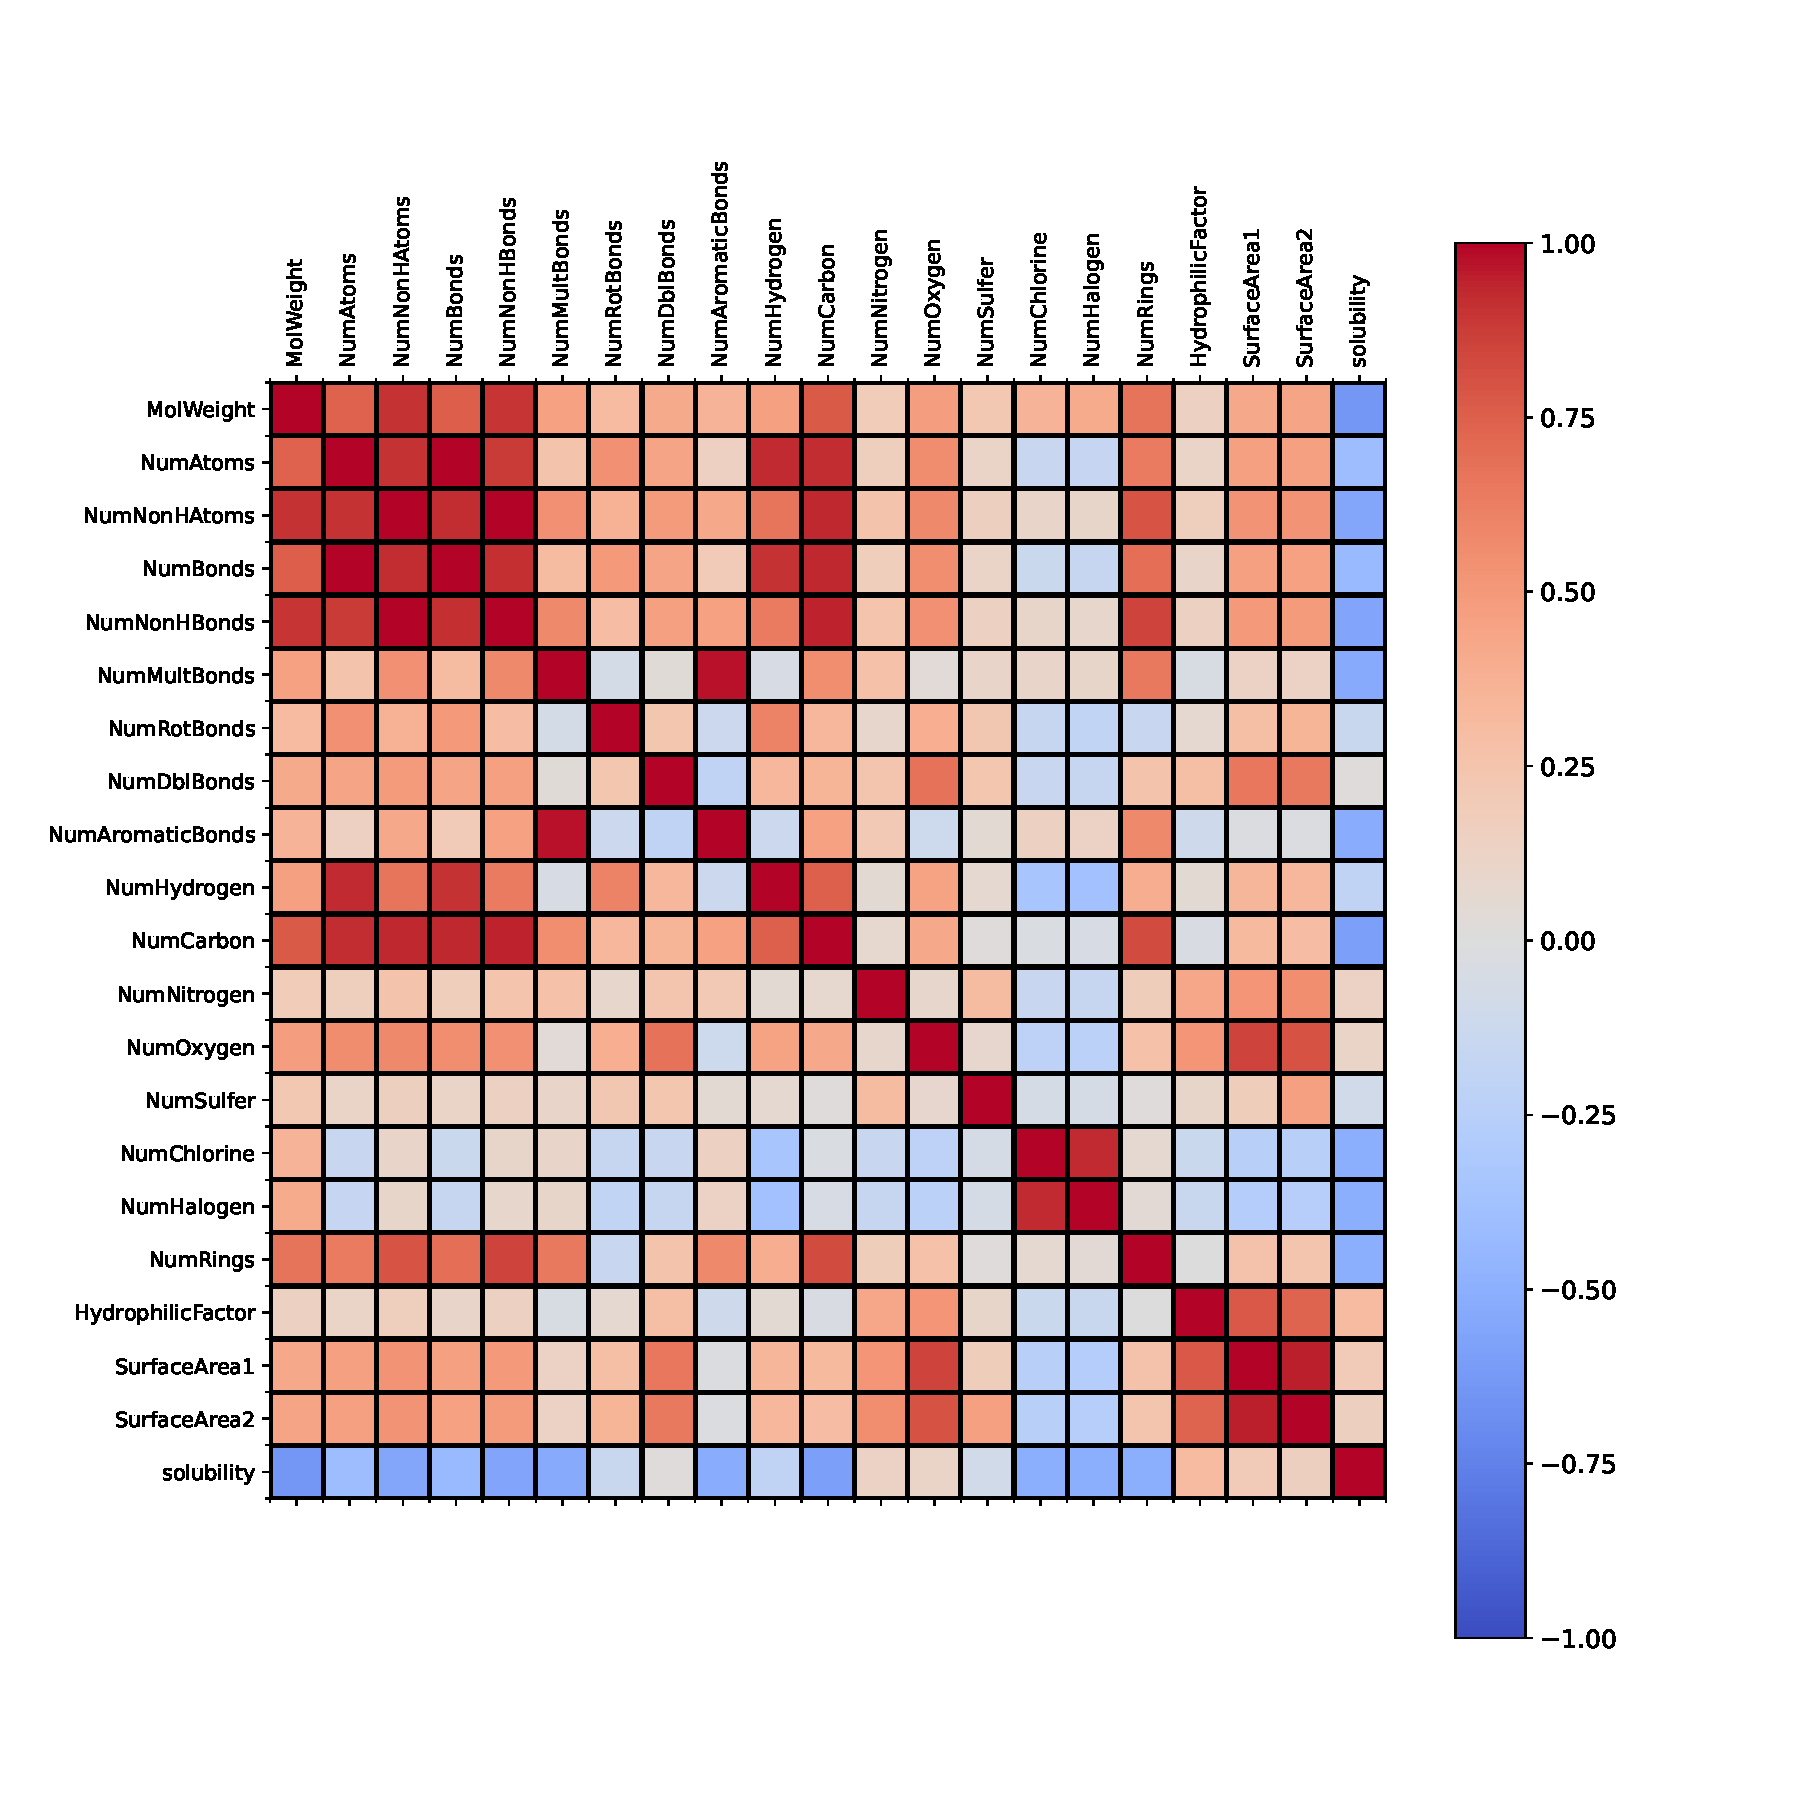
\includegraphics[width=0.55\textwidth]{../../code/hw2/figures/1-correlation_matrix.pdf}}
  \caption{Correlation Matrix presented as a Heatmap.}
  \label{fig:1-correlation_matrix}
\end{figure}

In order to provide data covariance in a understandable approach, we compute the covariance matrix and present it is a heatmap for visualization simplicity. Fig.~\ref{fig:1-correlation_matrix} shows that various predictors are strongly correlated, mainly positive.

\begin{figure}[htbp!]
  \centerline{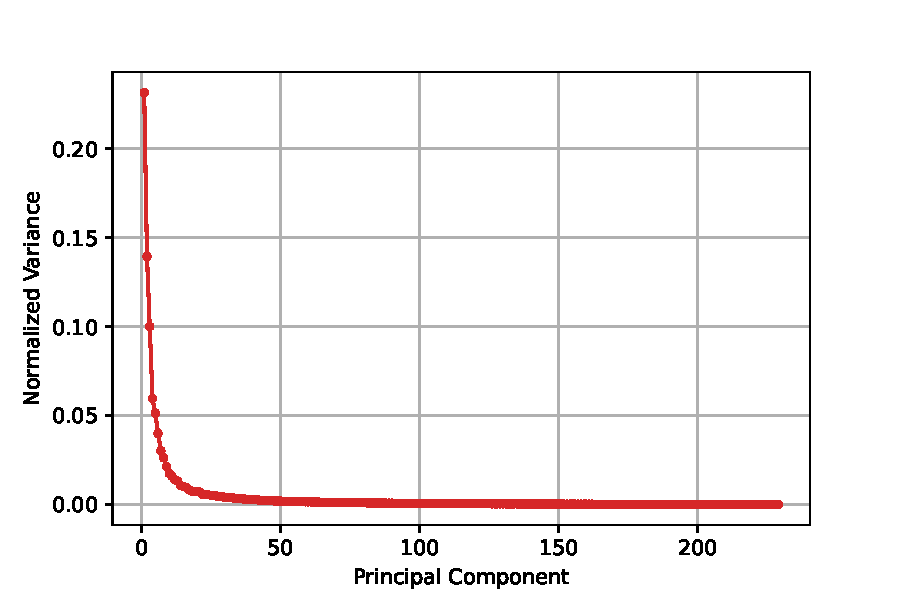
\includegraphics[width=0.52\textwidth]{../../code/hw2/figures/0-PCA-screeplot.pdf}}
  \caption{Screeplot showing the normalized variance, i.e, relevance, of each Principal Component.}
  \label{fig:0-PCA-screeplot}
\end{figure}

We can see in Fig.~\ref{fig:0-PCA-screeplot}, the normalized variance, i.e, relevance on our context vs. the principal components (PC). We also present a cumulative curve, which shows that the first 6 PC carries more than 60\% of the variance, leading to 95\% with 60 PC, what we can interprete as only 60 columns, i.e, 26\% of this dataset preserve 95\% from the original information. It means dividing the complexity by 3 and improving the storage and processing cost.

\subsection{Linear Regression Model}

For the first approach a simple regression model was implemented, using the eq.~\ref{eq:betas}. The results were reasonably satisfactory, showing a root mean square error (RMSE) of 0.467, and the $\text{R}^2$ statistic at 0.785. The graph comparing the values obtained from the model with those predicted is presented in the appendix, in figure~\ref{fig:2-linear-regression}. It is noticeable that there is a good clustering around the central line (which indicates the predicted value equal to the obtained one), but some points are relatively distant, and these happen relatively often. Therefore, it would be interesting to investigate whether with the same type of model this error could be reduced, demonstrating that these deviations are not only generated by the irreducible error.

\begin{figure}[htbp!]
  \centerline{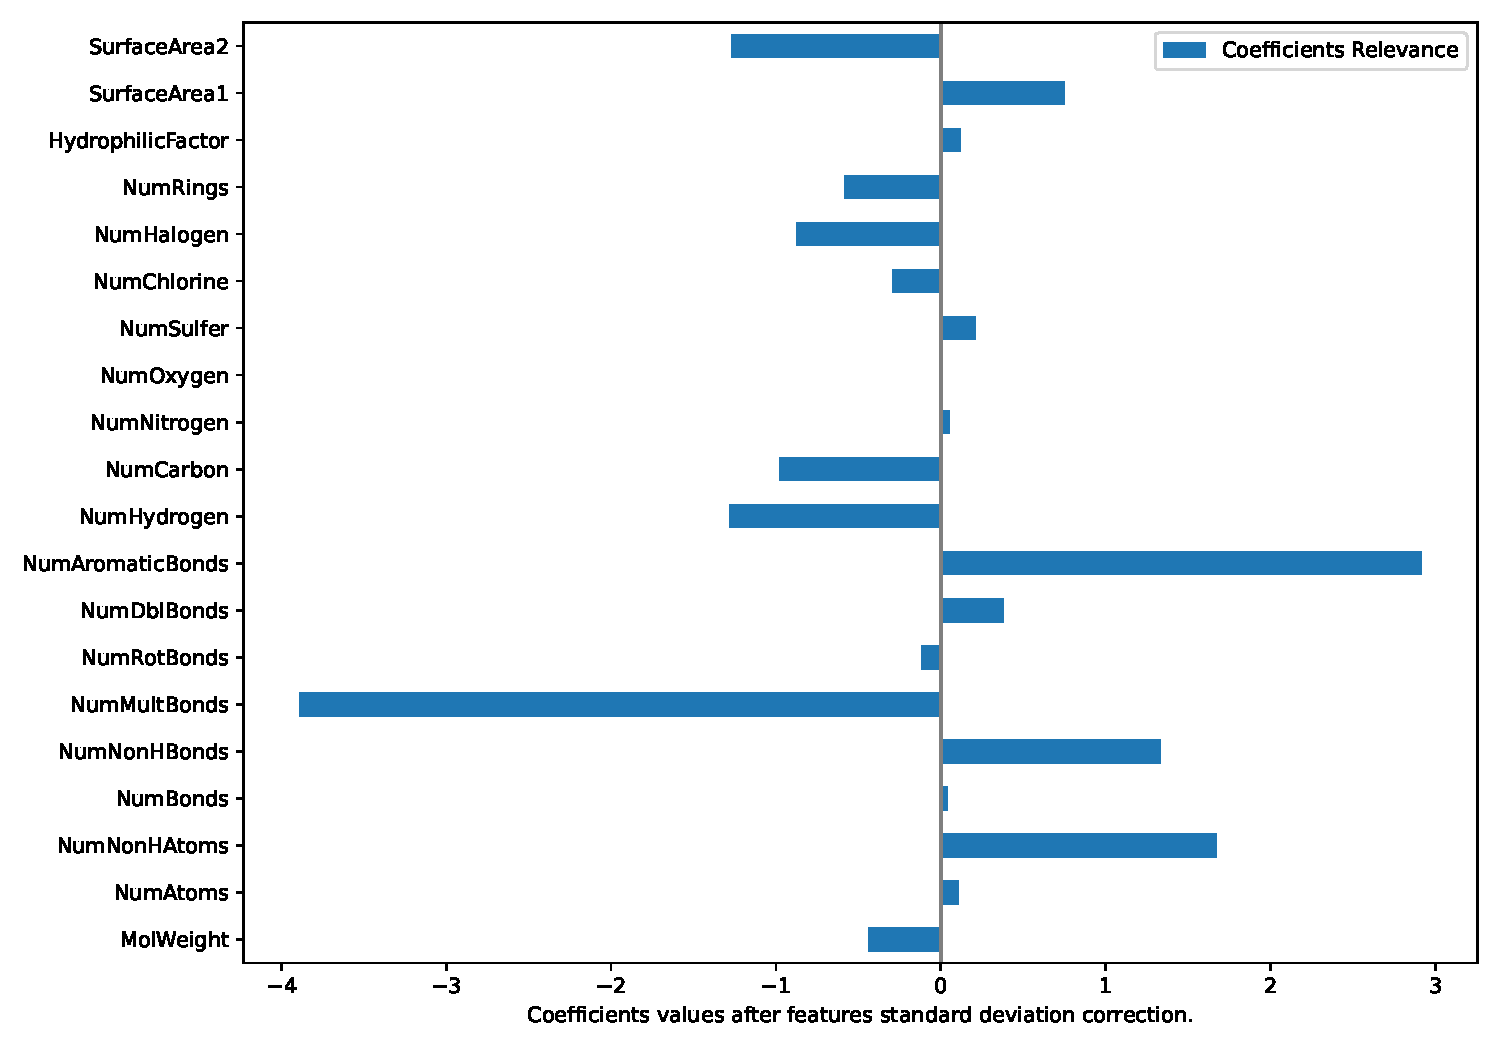
\includegraphics[width=0.5\textwidth]{../../code/hw2/figures/2-linear-regression-coefficients.pdf}}
  \caption{Linear regression coefficients.}
  \label{fig:2-linear-regression-coefficients}
\end{figure}

The linear coefficients after features standard deviation correction for non-binary data is presented in figure~\ref{fig:2-linear-regression-coefficients}. We may highlight two great coefficients for \textit{NumAromaticBonds} and \textit{NumMultBonds} predictors.

\subsection{Penalized Ridge Model}
The penalized model used in our experiments was the ``ridge regression'', which uses quadratic weights to compensate for the variances in the data, and slightly biases the data. Through cross-validation the optimal value of the factor $\lambda$ was determined to be 0.0286, in figure~\ref{fig:3-lambda-ridge}, having within the validation set in RMSE = 0.448. These results can be considered more interesting than the values obtained in the simple regression, but when applying the model to the test group, the generalization of the model did not obtain results as superior to simple regression, with RMSE = 0.474 and $\text{R}^2$ = 0.776. Although the performance on the test set was not as superior, the result obtained on the validation set indicates that there is likely to be better generalization ability, making the model present a better performance.

\begin{figure}[htbp!]
  \centerline{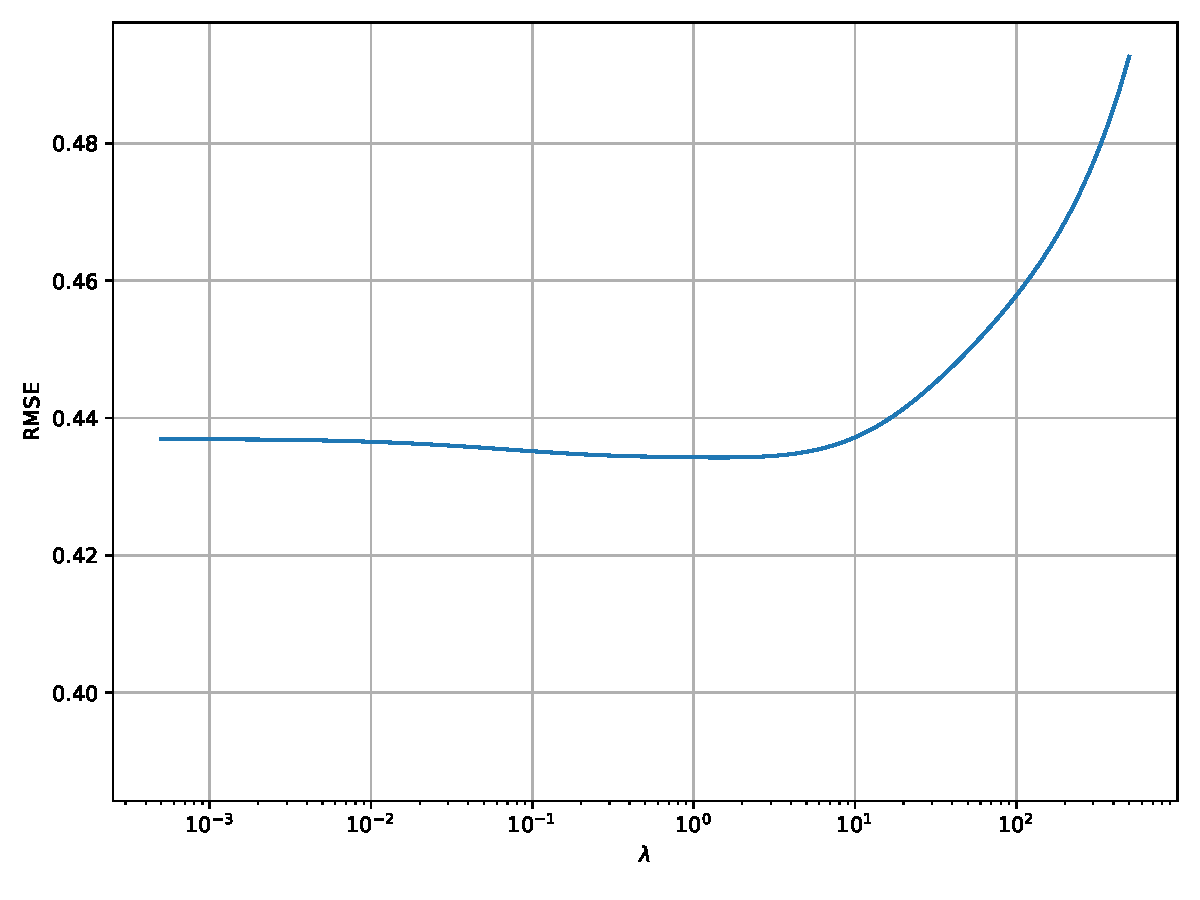
\includegraphics[width=0.5\textwidth]{../../code/hw2/figures/3-lambda-ridge.pdf}}
  \caption{$\lambda$ Parameter vs. RMSE for a Ridge Model.}
  \label{fig:3-lambda-ridge}
\end{figure}

There is also the option to increase even more the number of PCs used in the model to improve the RMSE, however it impacts on the model performance.

\subsection{Principal Component Regression}

\begin{figure}[htbp!]
  \centerline{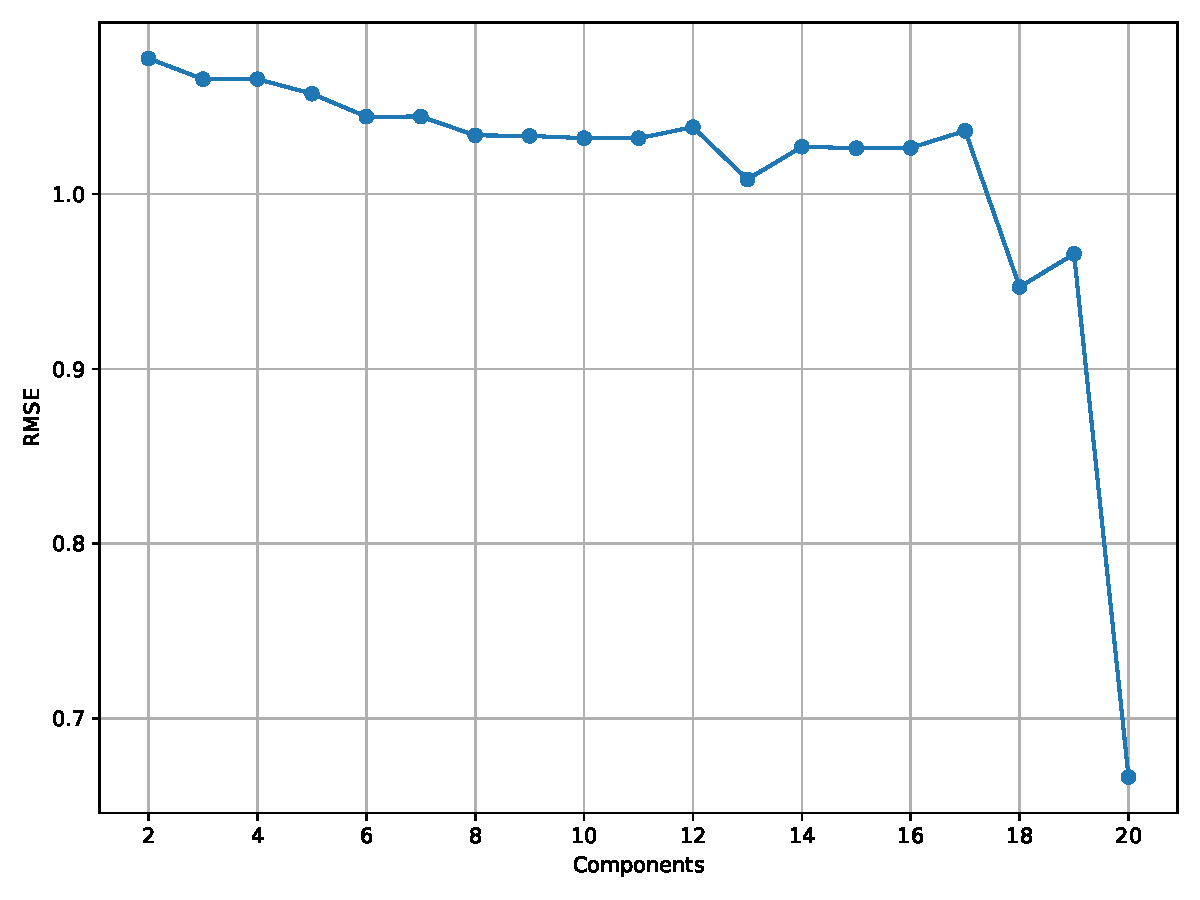
\includegraphics[width=0.5\textwidth]{../../code/hw2/figures/5-PCR-RMSE.pdf}}
  \caption{Components in the Model vs. RMSE for a PCR Model.}
  \label{fig:5-PCR-RMSE}
\end{figure}

\subsection{Partial Least Squares}

\begin{figure}[htbp!]
  \centerline{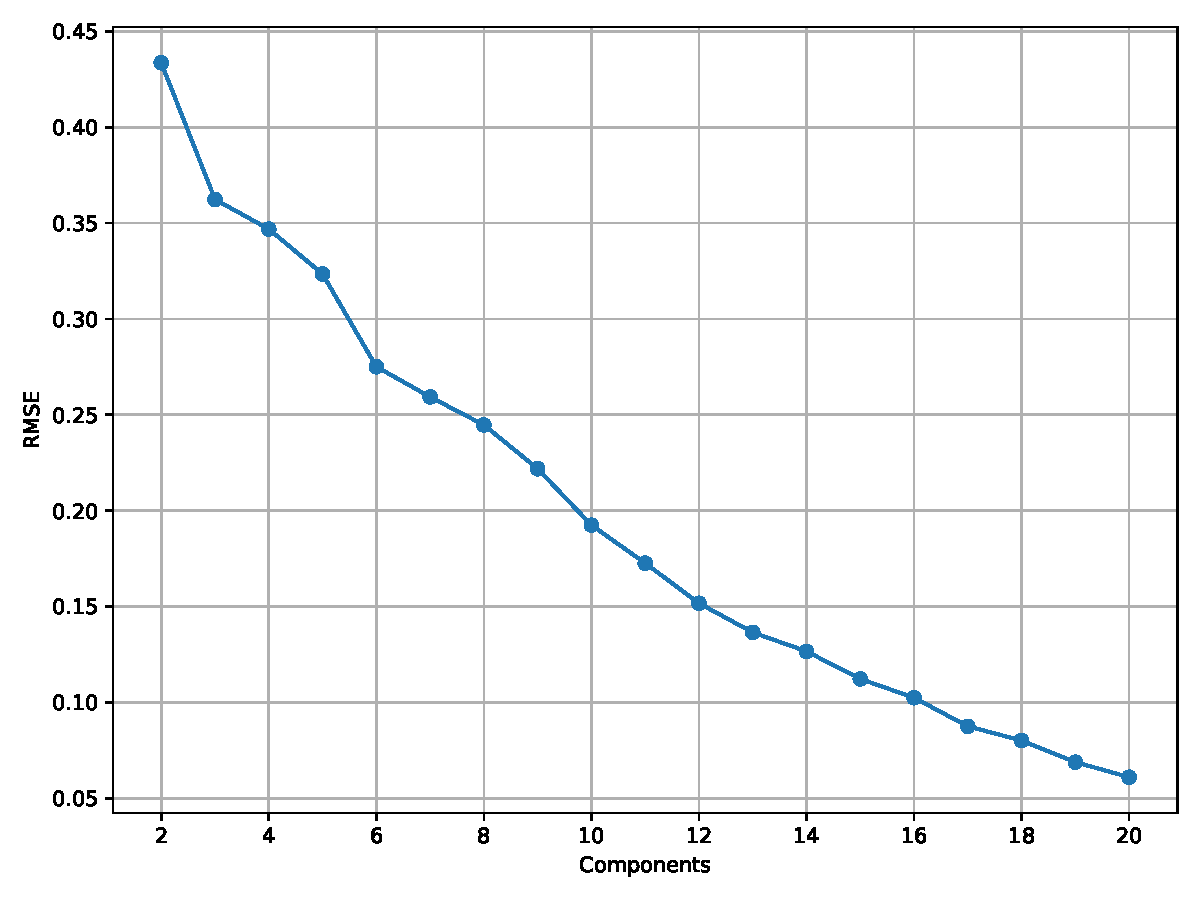
\includegraphics[width=0.5\textwidth]{../../code/hw2/figures/5-PLS-RMSE.pdf}}
  \caption{Components in the Model vs. RMSE for a PLS Model.}
  \label{fig:5-PLS-RMSE}
\end{figure}


% %paRTE 3
% \subsection{PCR e PLS}

% Como ultima abordagem para o desenvolvimento do modelo preditivo, foram desenvolvidos dois modelos que utilizam a redução de dimensão, o PCR e o PLS. Foram aplicados os algorítimos para a aplicação dos modelos, então comparados as precisões a medida que o número de dimensões dos modelos aumentavam.

% % \begin{figure}[h]
% %     \centering
% %     \captionsetup{justification = centering,margin=1cm}
% %     \caption{RMSE em PCR}
% %     \includegraphics[width=0.3\textwidth]{images/ComponentsxRMSE_PCR.pdf}
% %     \label{im:pcr}
% % \end{figure}

% Interessante observar que na figura (\ref{im:pcr}) nem sempre que há um aumento de dimensões há uma diminuição considerável do RMSE, nos permitindo inferir que algumas dessas dimensões não apresentam correlação com saída como descrito anteriormente. Vale ressaltar que o valor inicial também é relativamente elevado, e mesmo com 40 dimensões, a precisão atingida durante a validação cruzada foi de RMSE = 0.872 e $\text{R}^2$ = 0.821, valores inferiores ao resultados a aplicação no conjunto de teste com regressão simples. O maior agravante foi que a aplicação no conjunto de teste teve um resultado pior, com RMSE = 0.898 e $\text{R}^2$ = 0.813. Esses resultados nos levaram a concluir que a regressão em componentes independentes não é adequada para o problema proposto visto que soluções mais simples fornecem resultados melhores.

% % \begin{figure}[h]
% %     \centering
% %     \captionsetup{justification = centering,margin=1cm}
% %     \caption{RMSE em PLS}
% %     \includegraphics[width=0.3\textwidth]{images/ComponentsxRMSE_PLS.pdf}
% %     \label{im:pls}
% % \end{figure}

% Em seguida aplicamos a regressão em PLS, e obtivemos resultados mais otimistas. Ao realizar a validação cruzada, ilustrado na figura (\ref{im:pls}), obtivemos uma curva mais optimizada e com um número muito menor de dimensões que a PCR. Vale ressaltar que principalmente ao se adicionar as primeiras dimensões, temos reduções expressivas no RMSE, que tende a se estabilizar a medida que se ultrapassa 17 dimensões. Durante a a validação o melhor resultado (dentre as 20 dimensões) se deu com 19 dimensões, com RMSE = 0.695 e $\text{R}^2$ = 0.887. Esses número são claramente mais desejáveis que os obtidos via PCR, quanto aos obtidos no grupo de teste foram, RMSE = 0.732 e $\text{R}^2$ = 0.877, esses são suavemente superiores aos obtidos via regressão simples, o quais dependendo do banco de dados final ou da precisão necessária, provavelmente não compensarão o esforço computacional extra.